\documentclass[12pt,a4paper]{article}
\usepackage{amsmath,amscd,amsbsy,amssymb,latexsym,url,bm,amsthm}
\usepackage{epsfig,graphicx,subfigure}
\usepackage{enumitem,balance}
\usepackage{wrapfig}
\usepackage{mathrsfs,euscript}
\usepackage[usenames]{xcolor}
\usepackage{hyperref}
\usepackage[vlined,ruled,linesnumbered]{algorithm2e}
\hypersetup{colorlinks=true,linkcolor=black}

\newtheorem{theorem}{Theorem}
\newtheorem{lemma}[theorem]{Lemma}
\newtheorem{proposition}[theorem]{Proposition}
\newtheorem{corollary}[theorem]{Corollary}
\newtheorem{exercise}{Exercise}
\newtheorem*{solution}{Solution}
\newtheorem{definition}{Definition}
\theoremstyle{definition}

\renewcommand{\thefootnote}{\fnsymbol{footnote}}

\newcommand{\postscript}[2]
 {\setlength{\epsfxsize}{#2\hsize}
  \centerline{\epsfbox{#1}}}

\renewcommand{\baselinestretch}{1.0}

\setlength{\oddsidemargin}{-0.365in}
\setlength{\evensidemargin}{-0.365in}
\setlength{\topmargin}{-0.3in}
\setlength{\headheight}{0in}
\setlength{\headsep}{0in}
\setlength{\textheight}{10.1in}
\setlength{\textwidth}{7in}
\makeatletter \renewenvironment{proof}[1][Proof] {\par\pushQED{\qed}\normalfont\topsep6\p@\@plus6\p@\relax\trivlist\item[\hskip\labelsep\bfseries#1\@addpunct{.}]\ignorespaces}{\popQED\endtrivlist\@endpefalse} \makeatother
\makeatletter
\renewenvironment{solution}[1][Solution] {\par\pushQED{\qed}\normalfont\topsep6\p@\@plus6\p@\relax\trivlist\item[\hskip\labelsep\bfseries#1\@addpunct{.}]\ignorespaces}{\popQED\endtrivlist\@endpefalse} \makeatother

\begin{document}
\noindent

%========================================================================
\noindent\framebox[\linewidth]{\shortstack[c]{
\Large{\textbf{Lab03-Greedy Strategy}}\vspace{1mm}\\
CS214-Algorithm and Complexity, Xiaofeng Gao, Spring 2021.}}


\begin{center}
\footnotesize{\color{red}$*$ If there is any problem, please contact TA Haolin Zhou.}\par
% Please write down your name, student id and email.
\footnotesize{\color{blue}$*$ Name:Renyang Guan  \quad Student ID:519021911058 \quad Email: guanrenyang@sjtu.edu.cn}
\end{center}

\begin{enumerate}
	\item \textit{Interval Scheduling.} Interval Scheduling is a classic problem solved by \textbf{greedy algorithm}: given $n$ jobs and the $j$-th job starts at $s_j$ and finishes at $f_j$. Two jobs are compatible if they do not overlap. The goal is to find maximum subset of mutually compatible jobs. Tim wants to solve it by sort the jobs in descending order of $s_j$. Is this attempt correct? Prove the correctness of such idea, or else provide a counter-example.
	    \begin{solution}
	    Such idea is not true, the counter example is shown in Fig.~\ref{Fig-CounterExample}. The choice of the idea above will be $Job\quad 1$, while the optimal solution is the set of $\{Job\quad1,  Job\quad 2, Job\quad3,  Job \quad 4\}$.
	        
\begin{figure}[htbp]
    \centering
    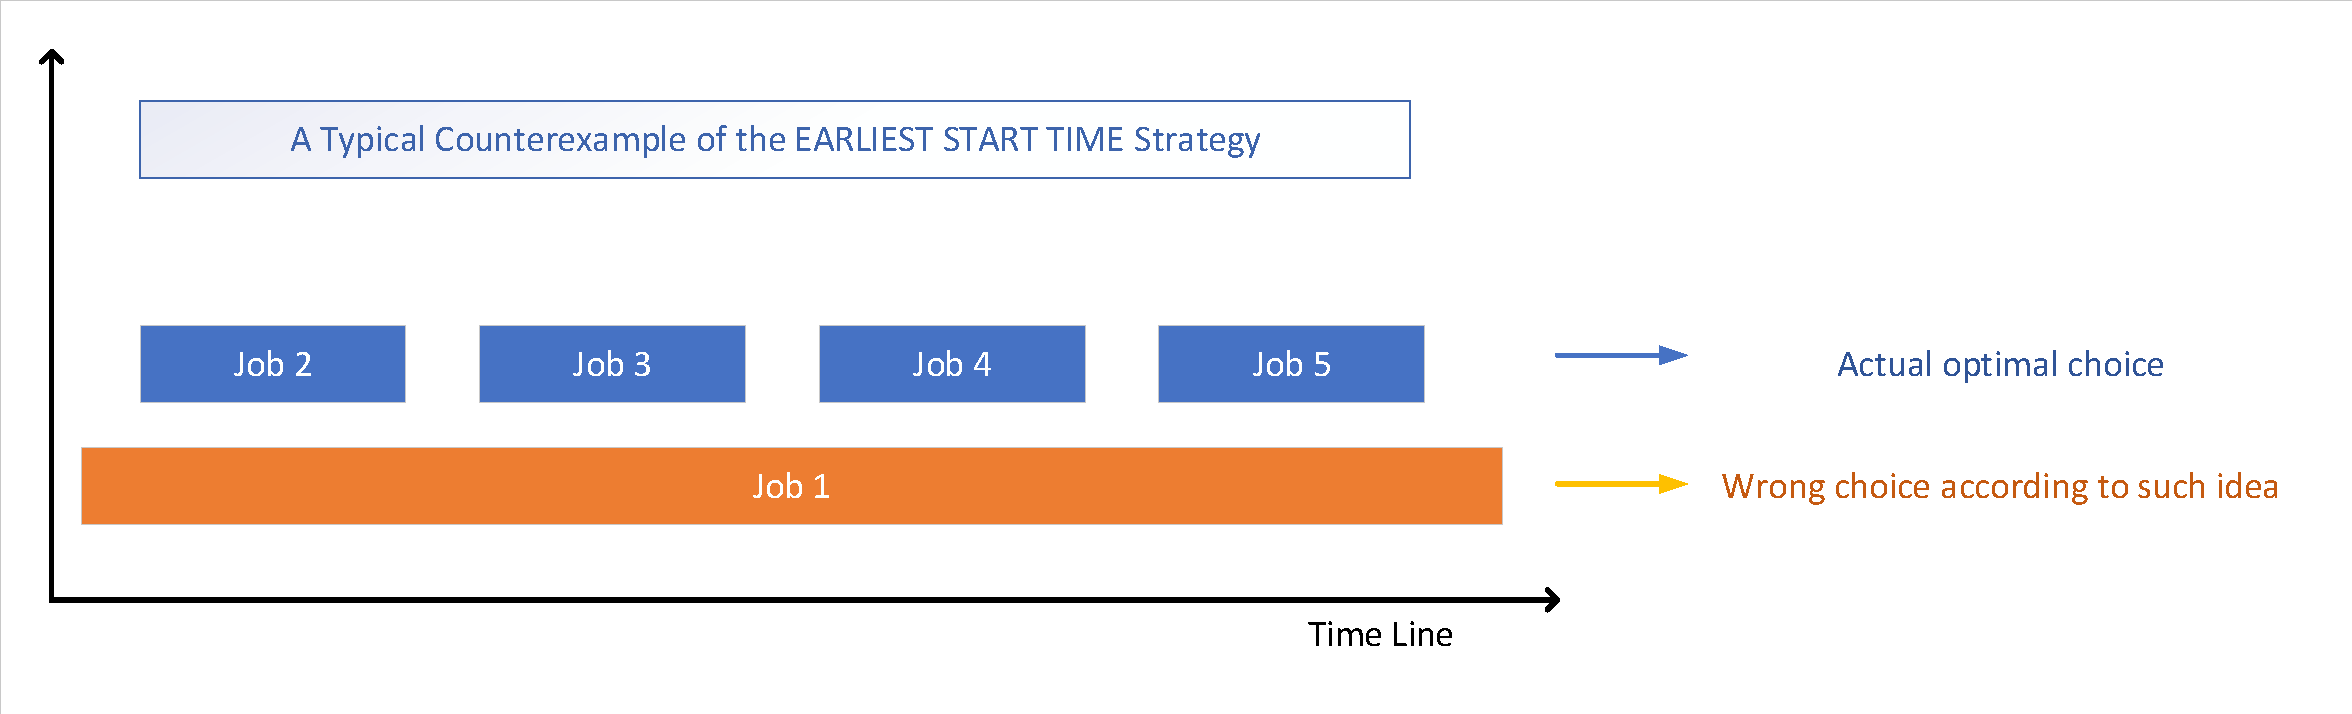
\includegraphics[width=0.8\textwidth]{Fig-CounterExample.pdf}
    \caption{A Typical Counterexample of the EARLIEST START TIME Strategy}\label{Fig-CounterExample}
\end{figure}
	    \end{solution}
	
	\item \textit{Done deal.} In a basketball league, teams need to complete player trades through matching contracts. Every player is offered a contract. For the sake of simplicity, we assume that the unit is $ M $, and the size of all contracts are integers. The process of contract matching refers to the equation: $ \sum_{i\in A} a_{i}=\sum_{j\in B} b_{j} $, where $ a_{i} $ refers to the contract value of player $ i $ in team $A$ involved in the trade and $ b_{j} $ refers to the value of player $ j $ in team $B$. 
	
	Assume that you are a manager of a basketball team and you want to get \textbf{one} star player from another team through trade. The contract of the star player is $ n (n\in \mathbb{N}^+) $. The goal is to complete the trade with as few players as possible. 
	
	\begin{enumerate}
		\item Describe a \textbf{greedy} algorithm to get the deal done with the least players in your team. Assume that there are only 4 types of contracts in your team: $25M$, $ 10M $, $ 5M $, $ 1M $, and there is no limit to the number of players. Prove that your algorithm yields an optimal solution.
		\item Suppose that the available contract sizes are powers of $c$,
		i.e., the values are $c^{0}, c^{1}, \ldots, c^{k}$ for some integers $c>1$ and $k \geq 1$. Show that the greedy algorithm always yields an optimal solution.
		\item Give a set of contract sizes for which the greedy algorithm does not yield an optimal solution. Your set should include a $ 1M $ so that there is a solution for every value of $ n $.
	\end{enumerate}
    \begin{solution}
    ~\\
    \begin{enumerate}
    \item 
    
    \textbf{\textit{Description of Algorithm: }} Let $S$ to be the set of all the player involved in the deal. The greedy algorithm asks to add the player with the highest contract value into $S$ when the adding operation won't make the sum of contract value of all players in $S$ exceeds $n$.
    \begin{proof}[Proof of Algorithm]
    ~\\
    \textbf{Notation:}
    \\
    \\
    \begin{tabular}{| c | l |}
    \hline
    Notation & Meaning of Notation \\
    \hline	
    $d(i)$ & Optimal solution with the sum of contract values is $n$\\
    $C$ & The biggest contract value that is smaller than $i$.
    \\
    \hline 

    \end{tabular}\\  
    \textbf{Greedy Choice:} Proving the its greedy choice is to prove : \textit{for each $d(i)$, $C$ must be in the global optimal solution}.
    
    If $C$ is not in the global optimal solution , this section of contract value has to be replaced by several players with smaller contract value. The number of players involved in the deal will increase after the replacement. 
    
    \textbf{Optimal Substructure:}Proving the optimal substructure is to prove $$d(i)=d(i-C)+1$$
    After dividing $i$ into $C$ and $i-C$, no player together with the player who has the contract value of $C$ could be replaced by a player having larger contract value. As a result, the optimal solution of $i-C$ together with $C$ is the optimal solution of $i$.
    \end{proof}
    
    \item
    
    \textbf{\textit{Notation:}}\\
    \begin{tabular}{| c | l |}
    \hline
    Notation & Meaning of Notation \\
    \hline
    $m_i$ & The number of players of a particular type of contract value.\\
    $T$ & The sum of contract values of  all players involved in a particular deal.\\
    $T_1$ & The solution of \textit{Greedy Algorithm}.\\
    $T_2$ & A solution of \textit{Non-Greedy Algorithm}\\
    $c$ & The smallest available contract size.\\
    \hline
    \end{tabular}
	\begin{proof}
	We could get the equation below from definition easily:
	\begin{equation}
	\begin{split}
	T_1=\sum_{i=0}^k m_i^1 c^i\\
	T_2=\sum_{i=0}^k m_i^2 c^i
	\end{split}
	\end{equation}
	Assume that $m_t^1\neq m_t^2$ while each $x>t$: $m_x^1=m_x^2$ and $m_t^1>m_t^2$, where $t$ could be any positive integer and $x$ is any positive integer bigger than $t$.
	We just need to consider the case where $m_t^1 - m_t^2 =1$:
	$$c^t=c^0+\sum_{i=0}^{t-1}(c-1)c^i >\sum_{i=0}^{t-1}(c-1)c^i$$
	$\forall i \in \{1,2,\cdots,k\}$, $\forall n\in \{1,2\}$:
	\begin{equation}
	\begin{split}
	& m_i^n<c\\
	& T_2=\sum_{i=0}^t m_i^2 c^i \leq \sum_{i=0}^{t-1}(c-1)c^i<c^t
	\end{split}
	\end{equation}
	So the rest of the contract value of players is smaller than $c^t$, $T_1$ is the global optimal solution.
	\end{proof}
	
	\item
	The set of contract is $$\{10M,9M,M\}$$
	If the contract value of the star is $n=18$. The solution of greedy algorithm is $18$ players while the optimal solution is $2$ players, both of whom have the contract value of $9M$.
    \end{enumerate}
    \end{solution}
	
    \item \textit{Set Cover.} \textbf{Set Cover} is a typical kind of problems that can be solved by greedy strategy. One version is that: Given $n$ points on a straight line, denoted as $\{x_i\}_{i=1}^n$, and we intend to use minimum number of closed intervals with fixed length $k$ to cover these $n$ points.
    \begin{enumerate}
    	\item Please design an algorithm based on \textbf{greedy} strategy to solve the above problem, in the form of \emph{pseudo code}. Then please analyze its \emph{worst-case} complexity.
    	\item Please prove the correctness of your algorithm.
    	\item Please complete the provided source code by C/C++ {\color{blue}(The source code \emph{Code-SetCover.cpp} is attached on the course webpage)}, and please write down the output result by testing the following inputs: 
    	\begin{enumerate}
    		\item the number of points $n=7$;
    		\item the coordinates of points
    		$x=\{1,2,3,4,5,6,-2\}$;
    		\item the length of intervals
    		$k=3$.
    	\end{enumerate}
        \textbf{Remark}: Screenshots of running results are also acceptable 
    \end{enumerate}
    \begin{solution}
    \begin{enumerate}
    \item
    \textbf{\texttt{Pseudo Code:}}\\
    \begin{algorithm}[H]
		\KwIn{An array $A[1,\cdots,n]$, integer $k$}
		\KwOut{$num\_interval$}
		
		\BlankLine
		\caption{Solution of Greedy Algorithm}\label{Alg-greedy}
		$num\_interval\leftarrow 0$\;
		sort $A[n]$ increasingly\;
		\For{$i\leftarrow 1$ \KwTo $n$}{
			\For{$j\leftarrow 0$ \KwTo $k$}{
				\If{$A[i]+j$ is in $A[1,2,\cdots,n]$}{
					$i\leftarrow (i+j)$\;				
				}			
			}	
			$num\_interval\leftarrow num\_interval+1$\;	
		}
		\Return{$num\_interval$}
	\end{algorithm}
    \textbf{\textit{Analysis of Worst Case Time Complexity:}}
    In all of the situations, the algorithm will only transverse the array once. The only difference to different input arrays is the step of i. The worst case occurs when $k$ is equivalent to $n$ and the interval of each pair of  adjacent elements in sorted $A$ is greater than $k$. Furthermore, the time complexity of sort is $O(n\log n)$.
    
    In this case, the \emph{for} loop in line 3 will loop for $n$ times and the inner \emph{for} loop in line 4 will loop for $k+1$ times. The best time complexity for search algorithm is $\Theta(\log n)$. Since 
    $$O((k+1)n\log n)+O(n\log n)=O(kn\log n)$$ 
    the time complexity of the algorithm is \textbf{$O(kn\log n)$}.
    \item
    \begin{proof}
    \textbf{\textit{Notation:}}\\
    \begin{tabular}{| c | l |}
    \hline    
    Notation & Meaning of Notation\\    
    \hline
    $X$ & Arbitrary set with integers.\\
    $d(X)$ & The optimal solution of covering the set $X$.\\
    $C$ & The greedy choice: the optimal solution of set $X/C$ is a subset of that of $X$.\\    
    \hline
    \end{tabular}
  	\\
  	\\
    \textbf{\textit{Greedy Choice:}}
    Proving the greedy choice is to prove: \textit{for each $d(X)$, $C$ must be in the global optimal solution}.
    
    If $C$ is not in the global optimal solution, the $k+1$ elements must be covered by more than one sets. 
        
    \textbf{\textit{Optimal Substructure:}}
    Proving the property of optimal substructure is to prove: 
    $$d(X)=d(X-C)+1$$
    Since every element in $C$ is smaller than any element in $X-C$, we could denote $C$ as $\{c_1,c_2,\cdots,c_j\}$, where $j\leq k+1$. There is no subset of $d(X-C)$ could cover all the elements of $C$ (If such an element exists, it will be covered by $C$.), so local optimal solution $d(X-C)$ is a subset of relatively global optimal solution $d(X)$. As a result of this, $d(X)$ equals to $d(X-C)$ plus the set $C$.
    
    \end{proof}
    
    \item The result of the test data is \emph{3} and the source code is in file \textit{Code-SetCover.cpp}.

    \end{enumerate}.
    \end{solution}
\end{enumerate}



\vspace{20pt}

\textbf{Remark:} You need to include your .pdf and .tex files in your uploaded .rar or .zip file.

%========================================================================
\end{document}
